\documentclass[crop,tikz]{standalone}
\usetikzlibrary{%
    arrows,
    arrows.meta,
    backgrounds,
    calc,
    decorations.pathreplacing,
    fit,
    matrix,
    positioning,
    scopes,
    shadows
}
\usepackage[linguistics]{forest}
\usepackage[charter]{mathdesign}
\tikzset{headarrow/.style = {-{Latex[length=.5em]}}}
\tikzset{move/.style = {dashed,blue,movearrow}}

\newcommand{\mlex}[2]{\ensuremath{\textrm{#1} ::\thinspace \mathrm{#2}}}
\newcommand{\fsel}[1]{\ensuremath{\mathrm{#1^+}}}
\newcommand{\fcat}[1]{\ensuremath{\mathrm{#1^-}}}
\newcommand{\flcr}[1]{\ensuremath{\mathrm{#1^+}}}
\newcommand{\flce}[1]{\ensuremath{\mathrm{#1^-}}}
\newcommand{\fadj}[1]{\ensuremath{\mathrm{#1^\sim}}}
\newcommand{\Merge}{Merge}
\newcommand{\Move}{Move}
\newcommand{\Adjoin}{Adjoin}

\begin{document}
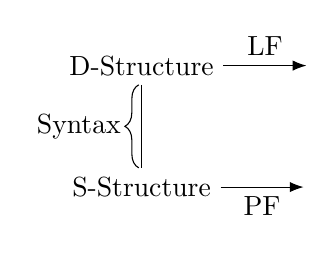
\begin{tikzpicture}[
    point/.style = {minimum size=0pt, inner sep=0pt, outer sep=0pt}]
    \node (start) at (0,0) {D-Structure};
    \node (end) [below=3em of start] {S-Structure};
    \node[point] (PF) [right=3em of end] {};
    \node[point] (LF) [right=3em of start] {};

    \draw (start) to (end);
    \draw[headarrow] (end) to node [below] {PF} (PF);
    \draw[headarrow] (start) to node [above] {LF} (LF);

    \draw[decorate,decoration={brace,amplitude=5pt,mirror}]
        ($(start.south) - (.1em,0)$)
        to
        node [left,xshift=-.3em] {Syntax}
        ($(end.north) - (.1em,0)$);
\end{tikzpicture}
\end{document}
